% vim: set spell spelllang=en tw=100 et sw=4 sts=4 foldmethod=marker foldmarker={{{,}}} :

\documentclass[aspectratio=169,compress,10pt]{beamer}

\usepackage{tikz}
\usepackage{xcolor}
\usepackage{complexity}
\usepackage{hyperref}
\usepackage{microtype}
\usepackage{amsmath}                   % \operatorname
\usepackage{amsfonts}                  % \mathcal
\usepackage{amssymb}                   % \nexists
\usepackage[vlined]{algorithm2e} % algorithms
\usepackage{centernot}
\usepackage{mathtools}
\usepackage{listings}

\usefonttheme{professionalfonts}

\usetikzlibrary{shapes, arrows, shadows, calc, positioning, fit}
\usetikzlibrary{decorations.pathreplacing, decorations.pathmorphing, shapes.misc}
\usetikzlibrary{tikzmark, backgrounds}

\definecolor{uofguniversityblue}{rgb}{0, 0.219608, 0.396078}

\definecolor{uofgheather}{rgb}{0.356863, 0.32549, 0.490196}
\definecolor{uofgaquamarine}{rgb}{0.603922, 0.72549, 0.678431}
\definecolor{uofgslate}{rgb}{0.309804, 0.34902, 0.380392}
\definecolor{uofgrose}{rgb}{0.823529, 0.470588, 0.709804}
\definecolor{uofgmocha}{rgb}{0.709804, 0.564706, 0.47451}
\definecolor{uofgsandstone}{rgb}{0.321569, 0.278431, 0.231373}
\definecolor{uofgforest}{rgb}{0, 0.2, 0.129412}
\definecolor{uofglawn}{rgb}{0.517647, 0.741176, 0}
\definecolor{uofgcobalt}{rgb}{0, 0.615686, 0.92549}
\definecolor{uofgturquoise}{rgb}{0, 0.709804, 0.819608}
\definecolor{uofgsunshine}{rgb}{1.0, 0.862745, 0.211765}
\definecolor{uofgpumpkin}{rgb}{1.0, 0.72549, 0.282353}
\definecolor{uofgthistle}{rgb}{0.584314, 0.070588, 0.447059}
\definecolor{uofgrust}{rgb}{0.603922, 0.227451, 0.023529}
\definecolor{uofgburgundy}{rgb}{0.490196, 0.133333, 0.223529}
\definecolor{uofgpillarbox}{rgb}{0.701961, 0.047059, 0}
\definecolor{uofglavendar}{rgb}{0.356863, 0.301961, 0.580392}

\tikzset{vertex/.style={draw, circle, inner sep=0pt, minimum size=0.5cm, font=\small\bfseries}}
\tikzset{notvertex/.style={vertex, color=white, text=black}}
\tikzset{plainvertex/.style={vertex}}
\tikzset{vertexc1/.style={vertex, fill=uofgburgundy, text=white}}
\tikzset{vertexc2/.style={vertex, fill=uofgsandstone, text=white}}
\tikzset{vertexc3/.style={vertex, fill=uofgforest, text=white}}
\tikzset{vertexc4/.style={vertex, fill=uofgheather, text=white}}
\tikzset{edge/.style={color=black!50!white}}
\tikzset{bedge/.style={ultra thick}}
\tikzset{edged/.style={color=screengrey, dashed}}
\tikzset{edgel3/.style={color=uofgrose, ultra thick}}

% {{{ theme things
\useoutertheme[footline=authortitle]{miniframes}
\useinnertheme{rectangles}

\setbeamerfont{block title}{size={}}
\setbeamerfont{title}{size=\large,series=\bfseries}
\setbeamerfont{section title}{size=\large,series=\mdseries}
\setbeamerfont{author}{size=\normalsize,series=\mdseries}
\setbeamercolor*{structure}{fg=uofguniversityblue}
\setbeamercolor*{palette primary}{use=structure,fg=black,bg=white}
\setbeamercolor*{palette secondary}{use=structure,fg=white,bg=uofgcobalt}
\setbeamercolor*{palette tertiary}{use=structure,fg=white,bg=uofguniversityblue}
\setbeamercolor*{palette quaternary}{fg=white,bg=black}
\setbeamercolor{block body}{bg=structure!10}
\setbeamercolor{block title}{bg=structure,fg=white}
\setbeamertemplate{blocks}[rounded]
\setbeamercolor*{titlelike}{parent=palette primary}

\beamertemplatenavigationsymbolsempty

\setbeamertemplate{title page}
{
    \begin{tikzpicture}[remember picture, overlay]
        \node at (current page.north west) {
            \begin{tikzpicture}[remember picture, overlay]
                \fill [fill=uofguniversityblue, anchor=north west] (0, 0) rectangle (\paperwidth, -2.6cm);
            \end{tikzpicture}
        };

        \node (logo) [anchor=north east, shift={(-0.8cm,-0.2cm)}] at (current page.north east) {
            
\includegraphics[keepaspectratio=true,scale=0.5]{UoG_keyline.pdf}
        };

        \node (logo2) [anchor=north, below=0.2cm of logo.south] {
            
\includegraphics[keepaspectratio=true,scale=0.1]{RAEngWhite.pdf}
        };

        \coordinate (logos) at ($(logo.south)!0.5!(logo2.north)$);

        \node [anchor=west, xshift=0.8cm] at (current page.west |- logos) {
            \begin{minipage}{0.65\paperwidth}\raggedright
                {\usebeamerfont{title}\usebeamercolor[white]{}\inserttitle}\\[0.1cm]
                {\usebeamerfont{author}\usebeamercolor[white]{}\insertauthor}
            \end{minipage}
        };
    \end{tikzpicture}
}

\setbeamertemplate{section page}
{
    \begin{centering}
        \begin{beamercolorbox}[sep=12pt,center]{part title}
            \usebeamerfont{section title}\insertsection\par
        \end{beamercolorbox}
    \end{centering}
}

\newcommand{\frameofframes}{/}
\newcommand{\setframeofframes}[1]{\renewcommand{\frameofframes}{#1}}

\makeatletter
\setbeamertemplate{footline}
{%
    \begin{beamercolorbox}[colsep=1.5pt]{upper separation line foot}
    \end{beamercolorbox}
    \begin{beamercolorbox}[ht=2.5ex,dp=1.125ex,%
        leftskip=.3cm,rightskip=.3cm plus1fil]{author in head/foot}%
        \leavevmode{\usebeamerfont{author in head/foot}\insertshortauthor}%
        \hfill%
        {\usebeamerfont{institute in head/foot}\usebeamercolor[fg]{institute in head/foot}\insertshortinstitute}%
    \end{beamercolorbox}%
    \begin{beamercolorbox}[ht=2.5ex,dp=1.125ex,%
        leftskip=.3cm,rightskip=.3cm plus1fil]{title in head/foot}%
        {\usebeamerfont{title in head/foot}\insertshorttitle}%
        \hfill%
        {\usebeamerfont{frame number}\usebeamercolor[fg]{frame number}\insertframenumber~\frameofframes~\inserttotalframenumber}
    \end{beamercolorbox}%
    \begin{beamercolorbox}[colsep=1.5pt]{lower separation line foot}
    \end{beamercolorbox}
}

\makeatletter
\setbeamertemplate{mini frame}
{%
  \begin{pgfpicture}{0pt}{0pt}{.04cm}{.04cm}
    \pgfpathcircle{\pgfpoint{0.04cm}{0.04cm}}{0.04cm}
    \pgfusepath{fill,stroke}
  \end{pgfpicture}%
}
\setbeamertemplate{mini frame in current subsection}
{%
  \begin{pgfpicture}{0pt}{0pt}{.04cm}{.04cm}
    \pgfpathcircle{\pgfpoint{0.04cm}{0.04cm}}{0.04cm}
    \pgfsetfillcolor{section in head/foot.bg}
    \pgfusepath{fill,stroke}
  \end{pgfpicture}%
}

\setbeamersize{mini frame size=0.10cm, mini frame offset=0.06cm}
\makeatother

% }}}

\title{Global Constraints and Consistency}
\author{Ciaran McCreesh}

\begin{document}

{
    \usebackgroundtemplate{
        \tikz[overlay, remember picture]
        \node[at=(current page.south), anchor=south, inner sep=0pt]{
\includegraphics[keepaspectratio=true, width=\paperwidth]{background1.jpg}};
    }
    \begin{frame}[plain,noframenumbering]
        \titlepage
    \end{frame}
}

\section{All-Different}

\begin{frame}{Two-Colouring a Triangle}

    \begin{columns}
        \begin{column}{0.45\textwidth}
            \begin{align*}
                & x_1 \in \{ 0, 1 \} \\
                & x_2 \in \{ 0, 1 \} \\
                & x_3 \in \{ 0, 1 \} \\
                & \mathrlap{\textit{alldifferent}( x_1, x_2, x_3 )} \\
                \\
                \\
            \end{align*}
        \end{column}
        \begin{column}{0.45\textwidth}
            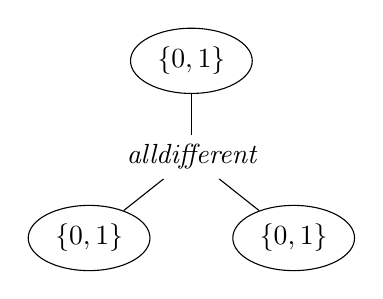
\begin{tikzpicture}
                \node [draw, ellipse] (C1) at (90:1.5) { $\{0,1\}$ };
                \node [draw, ellipse] (C2) at (210:1.5) { $\{0,1\}$ };
                \node [draw, ellipse] (C3) at (330:1.5) {  $\{0,1\}$  };

                \node [anchor = south] (C) at (0, 0) { $\textit{alldifferent}$ };

                \draw (C) to (C1);
                \draw (C) to (C2);
                \draw (C) to (C3);
            \end{tikzpicture}
        \end{column}
    \end{columns}

\end{frame}

\begin{frame}{Decomposing ``All Different''}

    \begin{columns}
        \begin{column}{0.45\textwidth}
            \begin{align*}
                & x_1 \in \{ 0, 1 \} \\
                & x_2 \in \{ 0, 1 \} \\
                & x_3 \in \{ 0, 1 \} \\
                & x_1 \ne x_2 \\
                & x_1 \ne x_3 \\
                & x_2 \ne x_3 \\
            \end{align*}
        \end{column}
        \begin{column}{0.45\textwidth}
            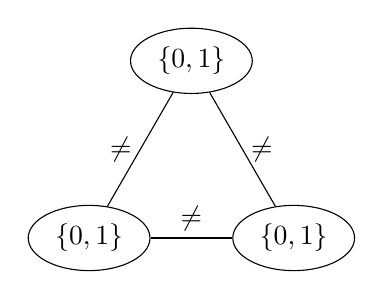
\begin{tikzpicture}
                \node [draw, ellipse] (C1) at (90:1.5) { $\{0,1\}$ };
                \node [draw, ellipse] (C2) at (210:1.5) { $\{0,1\}$ };
                \node [draw, ellipse] (C3) at (330:1.5) {  $\{0,1\}$  };

                \draw (C1) to node [xshift=-0.7em] { $\ne$ } (C2);
                \draw (C1) to node [xshift=0.7em] { $\ne$ } (C3);
                \draw (C2) to node [yshift=0.7em] { $\ne$ } (C3);
            \end{tikzpicture}
        \end{column}
    \end{columns}

\end{frame}

\begin{frame}{What Does Propagation Do?}

    \begin{itemize}
        \item Let's consider the constraint $x_1 \ne x_2$.
        \item Remember arc consistency: for each value, check whether it is supported by another
            value.
            \begin{itemize}
                \item If $x_1 = 0$, we can give $x_2 = 1$, so that's OK.
                \item If $x_1 = 1$, we can give $x_2 = 0$, so that's OK.
                \item If $x_2 = 0$, we can give $x_1 = 1$, so that's OK.
                \item If $x_2 = 1$, we can give $x_1 = 0$, so that's OK.
            \end{itemize}
        \item Let's consider the constraint $x_1 \ne x_3$.
            \begin{itemize}
                \item etc
            \end{itemize}
        \item Let's consider the constraint $x_2 \ne x_3$.
            \begin{itemize}
                \item etc
            \end{itemize}
        \item So no values are deleted, and everything looks OK.
    \end{itemize}
\end{frame}

\begin{frame}{What Does Propagation Really Do?}
    \begin{itemize}
        \item For a not-equals constraint, no need to call it at all until one of the variables
            has only one value remaining.
        \item Initial propagation literally does nothing!
    \end{itemize}
\end{frame}

\begin{frame}{What Would a Human Do?}
    \begin{center}
        ``Duh, obviously there's no solution! There \\ aren't enough numbers to go around.''
    \end{center}

    \begin{itemize}
        \item Unfortunately ``stare at it for a few seconds then write down the answer'' is not an algorithm.

        \item But if we don't decompose the constraint, we \emph{can} come up with a propagator
            which can tell that there's no solution.
    \end{itemize}
\end{frame}

\begin{frame}{Matchings and All-Different}

    \begin{columns}
        \begin{column}{0.76\textwidth}
            \begin{itemize}
                \item Draw a vertex on the left for each variable, and a vertex on the right for each value.
                \item Draw edges from each variable to each of its values.
                \item A \emph{maximum cardinality matching} is where you pick as many edges as
                    possible, but each vertex can only be used at most once.
                \item We can find this in polynomial time.
                \item There is a matching which covers each variable if and only if the constraint
                    can be satisfied.
                \item In fact, there is a one to one correspondence between
                    perfect matchings and solutions to the constraint.
            \end{itemize}
        \end{column}
        \begin{column}{0.22\textwidth}
            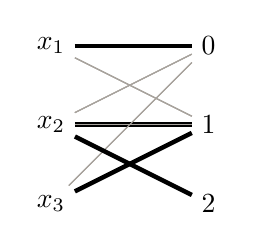
\begin{tikzpicture}
                \node (X1) at (0, 2) { $x_1$ };
                \node (X2) at (0, 1) { $x_2$ };
                \node (X3) at (0, 0) { $x_3$ };

                \node (V0) at (2, 2) { $0$ };
                \node (V1) at (2, 1) { $1$ };
                \node <3-> (V2) at (2, 0) { $2$ };

                \draw <1, 3> [color=uofgsandstone!50] (X1) -- (V0);
                \draw <1, 3> [color=uofgsandstone!50] (X1) -- (V1);
                \draw <1, 3> [color=uofgsandstone!50] (X2) -- (V0);
                \draw <1, 3> [color=uofgsandstone!50] (X2) -- (V1);
                \draw <1, 3> [color=uofgsandstone!50] (X3) -- (V0);
                \draw <1, 3> [color=uofgsandstone!50] (X3) -- (V1);
                \draw <3> [color=uofgsandstone!50] (X2) -- (V2);

                \draw <2> [color=uofgsandstone!50] (X1) -- (V1);
                \draw <2> [color=uofgsandstone!50] (X2) -- (V0);
                \draw <2> [color=uofgsandstone!50] (X3) -- (V0);
                \draw <2> [color=uofgsandstone!50] (X3) -- (V1);
                \draw <2> [ultra thick] (X1) -- (V0);
                \draw <2> [ultra thick] (X2) -- (V1);

                \draw <4> [color=uofgsandstone!50] (X1) -- (V1);
                \draw <4> [color=uofgsandstone!50] (X2) -- (V0);
                \draw <4> [color=uofgsandstone!50] (X2) -- (V1);
                \draw <4> [color=uofgsandstone!50] (X3) -- (V0);
                \draw <4> [ultra thick] (X1) -- (V0);
                \draw <4> [ultra thick] (X3) -- (V1);
                \draw <4> [ultra thick] (X2) -- (V2);
            \end{tikzpicture}
        \end{column}
    \end{columns}

\end{frame}

\begin{frame}{Sudoku}

    \centering
    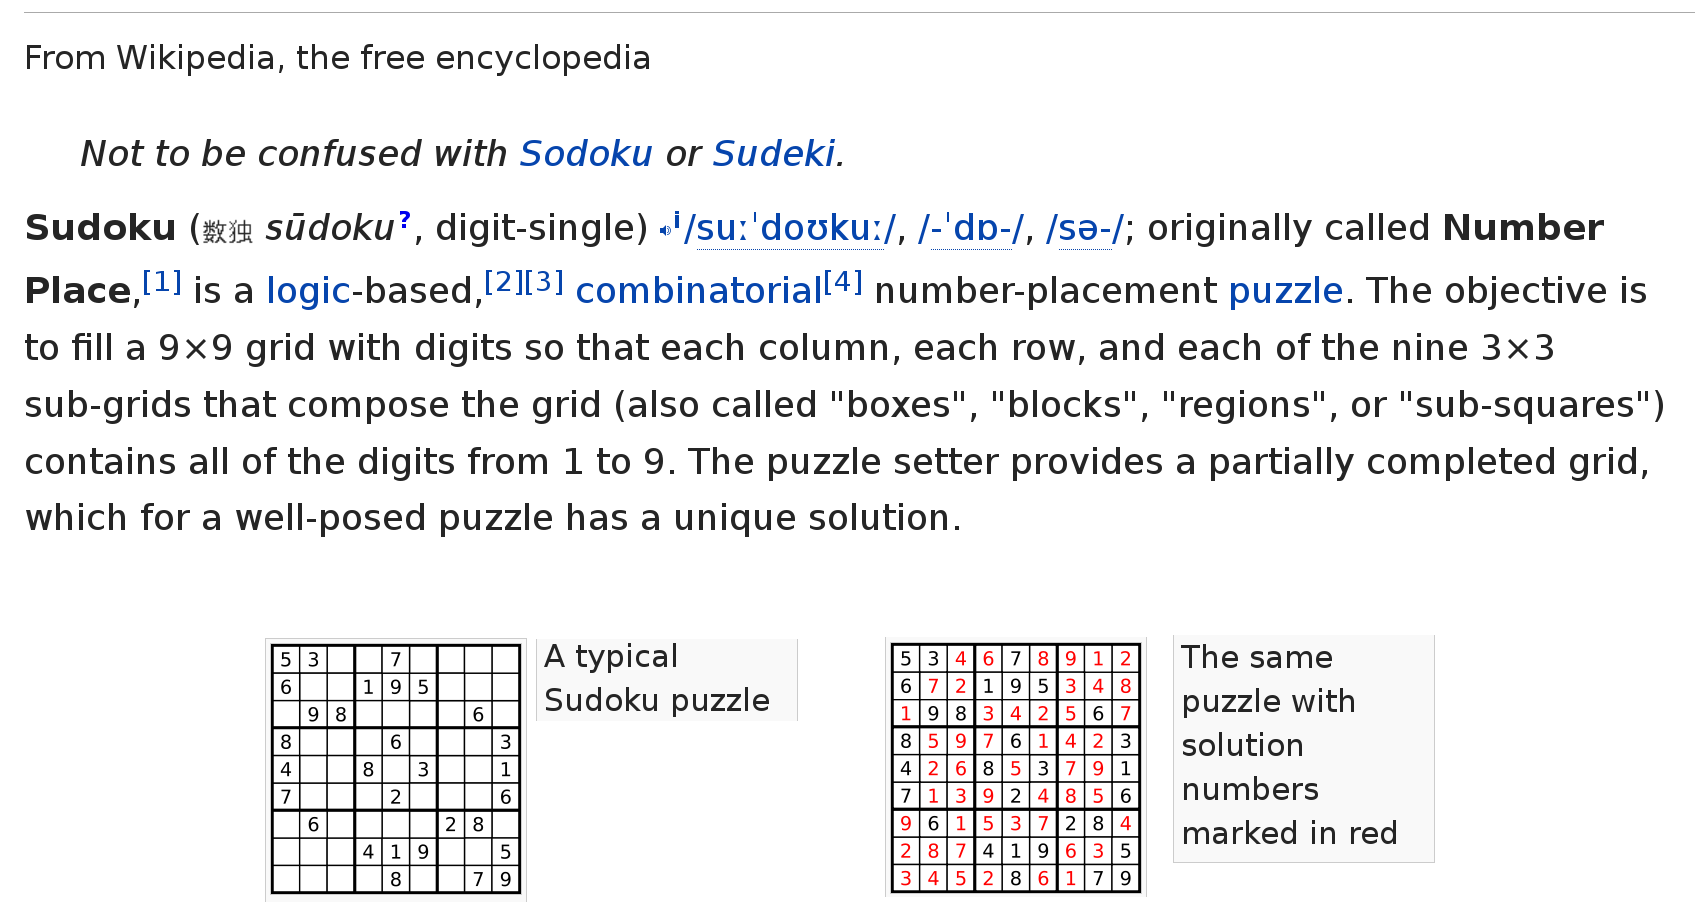
\includegraphics[keepaspectratio=true,scale=0.18]{sudoku.png}

\end{frame}

\begin{frame}{How do Humans Solve Sudoku?}
    \begin{center}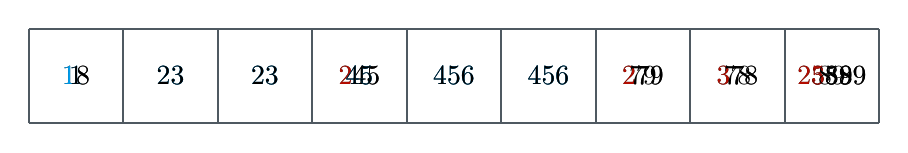
\begin{tikzpicture}[scale=0.4]
        \draw[thick, scale=3, color=uofgslate] (0, 0) grid (9, 1);

        \node <1>   [anchor=center] at (1.5, 1.5)  { 18 };
        \node <2>   [anchor=center] at (1.5, 1.5)  { \textcolor{uofgcobalt}{1}8 };
        \node <3>   [anchor=center] at (1.5, 1.5)  { \textcolor{uofgcobalt}{1} };
        \node <4->  [anchor=center] at (1.5, 1.5)  { 1 };

        \node <1-4> [anchor=center] at (4.5, 1.5)  { 23 };
        \node <5-6> [anchor=center] at (4.5, 1.5)  { \textcolor{uofgcobalt}{23} };
        \node <7->  [anchor=center] at (4.5, 1.5)  { 23 };

        \node <1-4> [anchor=center] at (7.5, 1.5)  { 23 };
        \node <5-6> [anchor=center] at (7.5, 1.5)  { \textcolor{uofgcobalt}{23} };
        \node <7->  [anchor=center] at (7.5, 1.5)  { 23 };

        \node <1-5> [anchor=center] at (10.5, 1.5) { 245 };
        \node <6>   [anchor=center] at (10.5, 1.5) { \textcolor{uofgpillarbox}{2}45 };
        \node <7>   [anchor=center] at (10.5, 1.5) { 45 };
        \node <8-9> [anchor=center] at (10.5, 1.5) { \textcolor{uofgcobalt}{45} };
        \node <10-> [anchor=center] at (10.5, 1.5) { 45 };

        \node <1-7> [anchor=center] at (13.5, 1.5) { 456 };
        \node <8-9>  [anchor=center] at (13.5, 1.5) { \textcolor{uofgcobalt}{456} };
        \node <10-> [anchor=center] at (13.5, 1.5) { 456 };

        \node <1-7> [anchor=center] at (16.5, 1.5) { 456 };
        \node <8-9> [anchor=center] at (16.5, 1.5) { \textcolor{uofgcobalt}{456} };
        \node <10-> [anchor=center] at (16.5, 1.5) { 456 };

        \node <1-5> [anchor=center] at (19.5, 1.5) { 279 };
        \node <6>   [anchor=center] at (19.5, 1.5) { \textcolor{uofgpillarbox}{2}79 };
        \node <7->  [anchor=center] at (19.5, 1.5) { 79 };

        \node <1-5> [anchor=center] at (22.5, 1.5) { 378 };
        \node <6>   [anchor=center] at (22.5, 1.5) { \textcolor{uofgpillarbox}{3}78 };
        \node <7->  [anchor=center] at (22.5, 1.5) { 78 };

        \node <1-5> [anchor=center] at (25.5, 1.5) { 23589 };
        \node <6>   [anchor=center] at (25.5, 1.5) { \textcolor{uofgpillarbox}{23}589 };
        \node <7-8> [anchor=center] at (25.5, 1.5) { 589 };
        \node <9>   [anchor=center] at (25.5, 1.5) { \textcolor{uofgpillarbox}{5}89 };
        \node <10-> [anchor=center] at (25.5, 1.5) { 89 };

    \end{tikzpicture}\end{center}
\end{frame}

\begin{frame}[fragile,t]{What Does A Constraint Solver Do?}
    \only<1> {
        If we work with a solver directly rather than using MiniZinc, we can propagate
        constraints and then stop, without searching. Here we'll use the Choco solver:
        \lstinputlisting[language=Java, basicstyle=\scriptsize\ttfamily,
        keywordstyle=\color{uofgcobalt}]{code/OneRow-snippet.java}
    }%
    \only<2> {
        \lstinputlisting[basicstyle=\scriptsize\ttfamily]{code/OneRow-output.txt}

        \begin{center}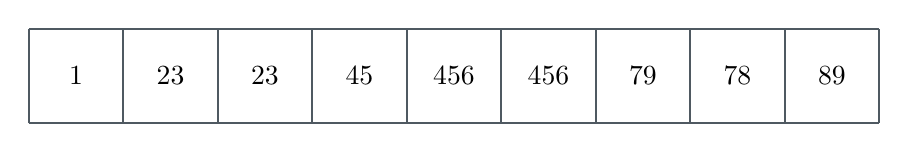
\begin{tikzpicture}[scale=0.4]
            \draw[thick, scale=3, color=uofgslate] (0, 0) grid (9, 1);

            \node [anchor=center] at (1.5, 1.5)  { 1 };
            \node [anchor=center] at (4.5, 1.5)  { 23 };
            \node [anchor=center] at (7.5, 1.5)  { 23 };
            \node [anchor=center] at (10.5, 1.5) { 45 };
            \node [anchor=center] at (13.5, 1.5) { 456 };
            \node [anchor=center] at (16.5, 1.5) { 456 };
            \node [anchor=center] at (19.5, 1.5) { 79 };
            \node [anchor=center] at (22.5, 1.5) { 78 };
            \node [anchor=center] at (25.5, 1.5) { 89 };

        \end{tikzpicture}\end{center}
    }%
    \only<3> {
        What if we used not-equals instead?

        \lstinputlisting[language=Java, basicstyle=\scriptsize\ttfamily,
        keywordstyle=\color{uofgcobalt}]{code/OneRowNeq-snippet.java}
    }%
    \only<4> {
        Remember that not-equals does nothing unless a variable has only one value remaining.

        \lstinputlisting[basicstyle=\scriptsize\ttfamily]{code/OneRowNeq-output.txt}
    }%
    \only<5-> {
        We could also get this through the MiniZinc IDE by selecting the Gecode Gist solver
        and using the ``Inspect'' tool, although it's a bit clumsy:

        \begin{center}
            \includegraphics<5>[scale=0.2]{gecode-gist-1.png}%
        \includegraphics<6>[scale=0.2]{gecode-gist-2.png}%
        \includegraphics<7>[scale=0.3]{gecode-gist-3.png}%

            \uncover<7>{Notice that Choco and Gecode do exactly the same thing. This is often not
            the case.}
        \end{center}
    }
\end{frame}

\begin{frame}{Generalised Arc Consistency}
    \begin{itemize}
        \item Arc Consistency (AC): for a binary constraint, each value is supported by at least one
            value in the other variable.
        \item Generalised Arc Consistency (GAC): for a global constraint, we can pick any value from any
            variable, and find a supporting set of values from each other variable in the constraint
            simultaneously.
            \begin{itemize}
                \item Each remaining value appears in at least one solution to the constraint.
            \end{itemize}
    \end{itemize}
\end{frame}

\begin{frame}{Hall Sets}
    \begin{itemize}
        \item A \emph{Hall set} of size $n$ is a set of $n$ variables from an ``all different''
            constraint, whose domains have $n$ values between them.

        \item If we can find a Hall set, we can safely remove these values from the domains of every
            other variable involved in the constraint.

        \item Hall's Marriage Theorem: doing this is equivalent to deleting every edge from the
            matching graph which cannot appear in any perfect matching.

        \item So, if we delete every Hall set, we delete every value that cannot appear in at least
            one way of satisfying the constraint. In other words, we obtain GAC.
    \end{itemize}
\end{frame}

\begin{frame}{Only Occurs in One Place?}

    \begin{center}
        ``But wait! We said that the value 1 only occurs \\
        in one place. That doesn't sound like a Hall set!''
    \end{center}

    \begin{itemize}
        \item <2-> The ``only occurs in one place'' rule we used first is just a Hall set of size 8.
    \end{itemize}
\end{frame}

\begin{frame}{GAC for All-Different}

    \only<1> {
        \begin{itemize}
            \item There are $2^n$ potential Hall sets, so considering them all is probably a bad
                idea\ldots
            \item Similarly, enumerating every perfect matching is \#P-hard.
            \item However, there is a polynomial algorithm! Here's a quick animation. For more, see
                one of the suggested poster papers.
        \end{itemize}
    }

    \only <2-12> {
        \begin{tikzpicture}[remember picture, overlay]
            \node (logo) [anchor=north east, shift={(-0.4cm,-0.8cm)}] at (current page.north east) {
                \begin{tikzpicture}[scale=0.25, font=\tiny]
                    \draw[thick, scale=3, color=uofgslate] (0, 0) grid (9, 1);
                    \node <2-11> [anchor=center] at (1.5, 1.5)  { 18 };
                    \node <2-11> [anchor=center] at (4.5, 1.5)  { 23 };
                    \node <2-11> [anchor=center] at (7.5, 1.5)  { 23 };
                    \node <2-11> [anchor=center] at (10.5, 1.5) { 245 };
                    \node <2-11> [anchor=center] at (13.5, 1.5) { 456 };
                    \node <2-11> [anchor=center] at (16.5, 1.5) { 456 };
                    \node <2-11> [anchor=center] at (19.5, 1.5) { 279 };
                    \node <2-11> [anchor=center] at (22.5, 1.5) { 378 };
                    \node <2-11> [anchor=center] at (25.5, 1.5) { 23589 };

                    \node <12> [anchor=center] at (1.5, 1.5)  { \textcolor{uofgcobalt}{1}\textcolor{uofgpillarbox}{8} };
                    \node <12> [anchor=center] at (4.5, 1.5)  { 23 };
                    \node <12> [anchor=center] at (7.5, 1.5)  { 23 };
                    \node <12> [anchor=center] at (10.5, 1.5) { \textcolor{uofgpillarbox}{2}45 };
                    \node <12> [anchor=center] at (13.5, 1.5) { 456 };
                    \node <12> [anchor=center] at (16.5, 1.5) { 456 };
                    \node <12> [anchor=center] at (19.5, 1.5) { \textcolor{uofgpillarbox}{2}79 };
                    \node <12> [anchor=center] at (22.5, 1.5) { \textcolor{uofgpillarbox}{3}78 };
                    \node <12> [anchor=center] at (25.5, 1.5) { \textcolor{uofgpillarbox}{235}89 };
                \end{tikzpicture}
            };
        \end{tikzpicture}%
        \centering
        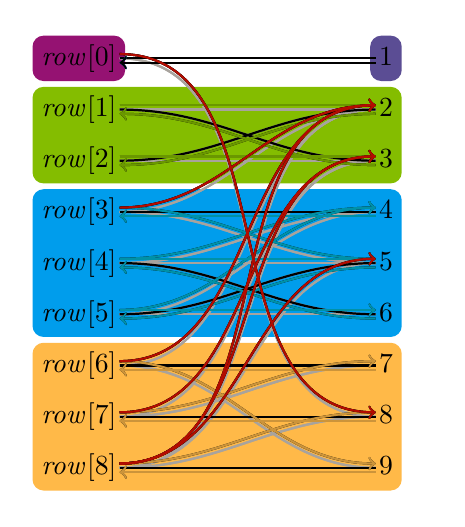
\begin{tikzpicture}[scale=0.65]
            \path (-1, -0.6) rectangle (7, 8.6);
            \node <3-> [inner sep = 1pt] (X1) at (0, 8) { $\mathit{row}[0]$ };
            \node <3-> [inner sep = 1pt] (X2) at (0, 7) { $\mathit{row}[1]$ };
            \node <3-> [inner sep = 1pt] (X3) at (0, 6) { $\mathit{row}[2]$ };
            \node <3-> [inner sep = 1pt] (X4) at (0, 5) { $\mathit{row}[3]$ };
            \node <3-> [inner sep = 1pt] (X5) at (0, 4) { $\mathit{row}[4]$ };
            \node <3-> [inner sep = 1pt] (X6) at (0, 3) { $\mathit{row}[5]$ };
            \node <3-> [inner sep = 1pt] (X7) at (0, 2) { $\mathit{row}[6]$ };
            \node <3-> [inner sep = 1pt] (X8) at (0, 1) { $\mathit{row}[7]$ };
            \node <3-> [inner sep = 1pt] (X9) at (0, 0) { $\mathit{row}[8]$ };

            \node <4-> [inner sep = 1pt] (V1) at (6, 8) { $1\vphantom{[]}$ };
            \node <4-> [inner sep = 1pt] (V2) at (6, 7) { $2\vphantom{[]}$ };
            \node <4-> [inner sep = 1pt] (V3) at (6, 6) { $3\vphantom{[]}$ };
            \node <4-> [inner sep = 1pt] (V4) at (6, 5) { $4\vphantom{[]}$ };
            \node <4-> [inner sep = 1pt] (V5) at (6, 4) { $5\vphantom{[]}$ };
            \node <4-> [inner sep = 1pt] (V6) at (6, 3) { $6\vphantom{[]}$ };
            \node <4-> [inner sep = 1pt] (V7) at (6, 2) { $7\vphantom{[]}$ };
            \node <4-> [inner sep = 1pt] (V8) at (6, 1) { $8\vphantom{[]}$ };
            \node <4-> [inner sep = 1pt] (V9) at (6, 0) { $9\vphantom{[]}$ };

            \draw <5> [thick, color=uofgsandstone!50] (X1.east) to [out=0, in=180] (V1.west);
            \draw <5> [thick, color=uofgsandstone!50] (X1.east) to [out=0, in=180] (V8.west);
            \draw <5> [thick, color=uofgsandstone!50] (X2.east) to [out=0, in=180] (V2.west);
            \draw <5> [thick, color=uofgsandstone!50] (X2.east) to [out=0, in=180] (V3.west);
            \draw <5> [thick, color=uofgsandstone!50] (X3.east) to [out=0, in=180] (V2.west);
            \draw <5> [thick, color=uofgsandstone!50] (X3.east) to [out=0, in=180] (V3.west);
            \draw <5> [thick, color=uofgsandstone!50] (X4.east) to [out=0, in=180] (V2.west);
            \draw <5> [thick, color=uofgsandstone!50] (X4.east) to [out=0, in=180] (V4.west);
            \draw <5> [thick, color=uofgsandstone!50] (X4.east) to [out=0, in=180] (V5.west);
            \draw <5> [thick, color=uofgsandstone!50] (X5.east) to [out=0, in=180] (V4.west);
            \draw <5> [thick, color=uofgsandstone!50] (X5.east) to [out=0, in=180] (V5.west);
            \draw <5> [thick, color=uofgsandstone!50] (X5.east) to [out=0, in=180] (V6.west);
            \draw <5> [thick, color=uofgsandstone!50] (X6.east) to [out=0, in=180] (V4.west);
            \draw <5> [thick, color=uofgsandstone!50] (X6.east) to [out=0, in=180] (V5.west);
            \draw <5> [thick, color=uofgsandstone!50] (X6.east) to [out=0, in=180] (V6.west);
            \draw <5> [thick, color=uofgsandstone!50] (X7.east) to [out=0, in=180] (V2.west);
            \draw <5> [thick, color=uofgsandstone!50] (X7.east) to [out=0, in=180] (V7.west);
            \draw <5> [thick, color=uofgsandstone!50] (X7.east) to [out=0, in=180] (V9.west);
            \draw <5> [thick, color=uofgsandstone!50] (X8.east) to [out=0, in=180] (V3.west);
            \draw <5> [thick, color=uofgsandstone!50] (X8.east) to [out=0, in=180] (V7.west);
            \draw <5> [thick, color=uofgsandstone!50] (X8.east) to [out=0, in=180] (V8.west);
            \draw <5> [thick, color=uofgsandstone!50] (X9.east) to [out=0, in=180] (V2.west);
            \draw <5> [thick, color=uofgsandstone!50] (X9.east) to [out=0, in=180] (V3.west);
            \draw <5> [thick, color=uofgsandstone!50] (X9.east) to [out=0, in=180] (V5.west);
            \draw <5> [thick, color=uofgsandstone!50] (X9.east) to [out=0, in=180] (V8.west);
            \draw <5> [thick, color=uofgsandstone!50] (X9.east) to [out=0, in=180] (V9.west);

            \draw <6> [thick, color=uofgsandstone!50] (X1.east) to [out=0, in=180] (V8.west);
            \draw <6> [thick, color=uofgsandstone!50] (X2.east) to [out=0, in=180] (V2.west);
            \draw <6> [thick, color=uofgsandstone!50] (X3.east) to [out=0, in=180] (V3.west);
            \draw <6> [thick, color=uofgsandstone!50] (X4.east) to [out=0, in=180] (V2.west);
            \draw <6> [thick, color=uofgsandstone!50] (X4.east) to [out=0, in=180] (V5.west);
            \draw <6> [thick, color=uofgsandstone!50] (X5.east) to [out=0, in=180] (V4.west);
            \draw <6> [thick, color=uofgsandstone!50] (X5.east) to [out=0, in=180] (V5.west);
            \draw <6> [thick, color=uofgsandstone!50] (X6.east) to [out=0, in=180] (V4.west);
            \draw <6> [thick, color=uofgsandstone!50] (X6.east) to [out=0, in=180] (V6.west);
            \draw <6> [thick, color=uofgsandstone!50] (X7.east) to [out=0, in=180] (V2.west);
            \draw <6> [thick, color=uofgsandstone!50] (X7.east) to [out=0, in=180] (V9.west);
            \draw <6> [thick, color=uofgsandstone!50] (X8.east) to [out=0, in=180] (V3.west);
            \draw <6> [thick, color=uofgsandstone!50] (X8.east) to [out=0, in=180] (V7.west);
            \draw <6> [thick, color=uofgsandstone!50] (X9.east) to [out=0, in=180] (V2.west);
            \draw <6> [thick, color=uofgsandstone!50] (X9.east) to [out=0, in=180] (V3.west);
            \draw <6> [thick, color=uofgsandstone!50] (X9.east) to [out=0, in=180] (V5.west);
            \draw <6> [thick, color=uofgsandstone!50] (X9.east) to [out=0, in=180] (V8.west);
            \draw <6> [thick] (X9.east) to [out=0, in=180] (V9.west);
            \draw <6> [thick] (X1.east) to [out=0, in=180] (V1.west);
            \draw <6> [thick] (X2.east) to [out=0, in=180] (V3.west);
            \draw <6> [thick] (X3.east) to [out=0, in=180] (V2.west);
            \draw <6> [thick] (X4.east) to [out=0, in=180] (V4.west);
            \draw <6> [thick] (X5.east) to [out=0, in=180] (V6.west);
            \draw <6> [thick] (X6.east) to [out=0, in=180] (V5.west);
            \draw <6> [thick] (X7.east) to [out=0, in=180] (V7.west);
            \draw <6> [thick] (X8.east) to [out=0, in=180] (V8.west);

            \draw <7-8> [thick, ->] ($(X1.east)!0.25!(X1.north east)$) to [out=0, in=180] ($(V8.west)!0.25!(V8.north west)$);
            \draw <7-8> [thick, ->] ($(X2.east)!0.25!(X2.north east)$) to [out=0, in=180] ($(V2.west)!0.25!(V2.north west)$);
            \draw <7-8> [thick, ->] ($(X3.east)!0.25!(X3.north east)$) to [out=0, in=180] ($(V3.west)!0.25!(V3.north west)$);
            \draw <7-8> [thick, ->] ($(X4.east)!0.25!(X4.north east)$) to [out=0, in=180] ($(V2.west)!0.25!(V2.north west)$);
            \draw <7-8> [thick, ->] ($(X4.east)!0.25!(X4.north east)$) to [out=0, in=180] ($(V5.west)!0.25!(V5.north west)$);
            \draw <7-8> [thick, ->] ($(X5.east)!0.25!(X5.north east)$) to [out=0, in=180] ($(V4.west)!0.25!(V4.north west)$);
            \draw <7-8> [thick, ->] ($(X5.east)!0.25!(X5.north east)$) to [out=0, in=180] ($(V5.west)!0.25!(V5.north west)$);
            \draw <7-8> [thick, ->] ($(X6.east)!0.25!(X6.north east)$) to [out=0, in=180] ($(V4.west)!0.25!(V4.north west)$);
            \draw <7-8> [thick, ->] ($(X6.east)!0.25!(X6.north east)$) to [out=0, in=180] ($(V6.west)!0.25!(V6.north west)$);
            \draw <7-8> [thick, ->] ($(X7.east)!0.25!(X7.north east)$) to [out=0, in=180] ($(V2.west)!0.25!(V2.north west)$);
            \draw <7-8> [thick, ->] ($(X7.east)!0.25!(X7.north east)$) to [out=0, in=180] ($(V9.west)!0.25!(V9.north west)$);
            \draw <7-8> [thick, ->] ($(X8.east)!0.25!(X8.north east)$) to [out=0, in=180] ($(V3.west)!0.25!(V3.north west)$);
            \draw <7-8> [thick, ->] ($(X8.east)!0.25!(X8.north east)$) to [out=0, in=180] ($(V7.west)!0.25!(V7.north west)$);
            \draw <7-8> [thick, ->] ($(X9.east)!0.25!(X9.north east)$) to [out=0, in=180] ($(V2.west)!0.25!(V2.north west)$);
            \draw <7-8> [thick, ->] ($(X9.east)!0.25!(X9.north east)$) to [out=0, in=180] ($(V3.west)!0.25!(V3.north west)$);
            \draw <7-8> [thick, ->] ($(X9.east)!0.25!(X9.north east)$) to [out=0, in=180] ($(V5.west)!0.25!(V5.north west)$);
            \draw <7-8> [thick, ->] ($(X9.east)!0.25!(X9.north east)$) to [out=0, in=180] ($(V8.west)!0.25!(V8.north west)$);
            \draw <7-8> [thick, <-] ($(X9.east)!0.25!(X9.south east)$) to [out=0, in=180] ($(V9.west)!0.25!(V9.south west)$);
            \draw <7-8> [thick, <-] ($(X1.east)!0.25!(X1.south east)$) to [out=0, in=180] ($(V1.west)!0.25!(V1.south west)$);
            \draw <7-8> [thick, <-] ($(X2.east)!0.25!(X2.south east)$) to [out=0, in=180] ($(V3.west)!0.25!(V3.south west)$);
            \draw <7-8> [thick, <-] ($(X3.east)!0.25!(X3.south east)$) to [out=0, in=180] ($(V2.west)!0.25!(V2.south west)$);
            \draw <7-8> [thick, <-] ($(X4.east)!0.25!(X4.south east)$) to [out=0, in=180] ($(V4.west)!0.25!(V4.south west)$);
            \draw <7-8> [thick, <-] ($(X5.east)!0.25!(X5.south east)$) to [out=0, in=180] ($(V6.west)!0.25!(V6.south west)$);
            \draw <7-8> [thick, <-] ($(X6.east)!0.25!(X6.south east)$) to [out=0, in=180] ($(V5.west)!0.25!(V5.south west)$);
            \draw <7-8> [thick, <-] ($(X7.east)!0.25!(X7.south east)$) to [out=0, in=180] ($(V7.west)!0.25!(V7.south west)$);
            \draw <7-8> [thick, <-] ($(X8.east)!0.25!(X8.south east)$) to [out=0, in=180] ($(V8.west)!0.25!(V8.south west)$);

            \draw <9> [thick, ->, color=uofglawn!80!black] ($(X2.east)!0.25!(X2.north east)$) to [out=0, in=180] ($(V2.west)!0.25!(V2.north west)$);
            \draw <9> [thick, ->, color=uofglawn!80!black] ($(X3.east)!0.25!(X3.north east)$) to [out=0, in=180] ($(V3.west)!0.25!(V3.north west)$);
            \draw <9> [thick, <-, color=uofglawn!80!black] ($(X2.east)!0.25!(X2.south east)$) to [out=0, in=180] ($(V3.west)!0.25!(V3.south west)$);
            \draw <9> [thick, <-, color=uofglawn!80!black] ($(X3.east)!0.25!(X3.south east)$) to [out=0, in=180] ($(V2.west)!0.25!(V2.south west)$);
            \draw <9> [thick, ->, color=uofgturquoise!80!black] ($(X4.east)!0.25!(X4.north east)$) to [out=0, in=180] ($(V5.west)!0.25!(V5.north west)$);
            \draw <9> [thick, ->, color=uofgturquoise!80!black] ($(X5.east)!0.25!(X5.north east)$) to [out=0, in=180] ($(V4.west)!0.25!(V4.north west)$);
            \draw <9> [thick, ->, color=uofgturquoise!80!black] ($(X5.east)!0.25!(X5.north east)$) to [out=0, in=180] ($(V5.west)!0.25!(V5.north west)$);
            \draw <9> [thick, ->, color=uofgturquoise!80!black] ($(X6.east)!0.25!(X6.north east)$) to [out=0, in=180] ($(V4.west)!0.25!(V4.north west)$);
            \draw <9> [thick, ->, color=uofgturquoise!80!black] ($(X6.east)!0.25!(X6.north east)$) to [out=0, in=180] ($(V6.west)!0.25!(V6.north west)$);
            \draw <9> [thick, <-, color=uofgturquoise!80!black] ($(X4.east)!0.25!(X4.south east)$) to [out=0, in=180] ($(V4.west)!0.25!(V4.south west)$);
            \draw <9> [thick, <-, color=uofgturquoise!80!black] ($(X5.east)!0.25!(X5.south east)$) to [out=0, in=180] ($(V6.west)!0.25!(V6.south west)$);
            \draw <9> [thick, <-, color=uofgturquoise!80!black] ($(X6.east)!0.25!(X6.south east)$) to [out=0, in=180] ($(V5.west)!0.25!(V5.south west)$);
            \draw <9> [thick, ->, color=uofgpumpkin!80!black] ($(X7.east)!0.25!(X7.north east)$) to [out=0, in=180] ($(V9.west)!0.25!(V9.north west)$);
            \draw <9> [thick, ->, color=uofgpumpkin!80!black] ($(X8.east)!0.25!(X8.north east)$) to [out=0, in=180] ($(V7.west)!0.25!(V7.north west)$);
            \draw <9> [thick, ->, color=uofgpumpkin!80!black] ($(X9.east)!0.25!(X9.north east)$) to [out=0, in=180] ($(V8.west)!0.25!(V8.north west)$);
            \draw <9> [thick, <-, color=uofgpumpkin!80!black] ($(X9.east)!0.25!(X9.south east)$) to [out=0, in=180] ($(V9.west)!0.25!(V9.south west)$);
            \draw <9> [thick, <-, color=uofgpumpkin!80!black] ($(X7.east)!0.25!(X7.south east)$) to [out=0, in=180] ($(V7.west)!0.25!(V7.south west)$);
            \draw <9> [thick, <-, color=uofgpumpkin!80!black] ($(X8.east)!0.25!(X8.south east)$) to [out=0, in=180] ($(V8.west)!0.25!(V8.south west)$);
            \draw <11-> [thick, <-, color=uofgcobalt] ($(X1.east)!0.25!(X1.south east)$) to [out=0, in=180] ($(V1.west)!0.25!(V1.south west)$);
            \draw <9-10>  [thick, <-] ($(X1.east)!0.25!(X1.south east)$) to [out=0, in=180] ($(V1.west)!0.25!(V1.south west)$);
            \draw <9-10>  [thick, ->] ($(X4.east)!0.25!(X4.north east)$) to [out=0, in=180] ($(V2.west)!0.25!(V2.north west)$);
            \draw <9-10>  [thick, ->] ($(X7.east)!0.25!(X7.north east)$) to [out=0, in=180] ($(V2.west)!0.25!(V2.north west)$);
            \draw <9-10>  [thick, ->] ($(X8.east)!0.25!(X8.north east)$) to [out=0, in=180] ($(V3.west)!0.25!(V3.north west)$);
            \draw <9-10>  [thick, ->] ($(X9.east)!0.25!(X9.north east)$) to [out=0, in=180] ($(V2.west)!0.25!(V2.north west)$);
            \draw <9-10>  [thick, ->] ($(X9.east)!0.25!(X9.north east)$) to [out=0, in=180] ($(V3.west)!0.25!(V3.north west)$);
            \draw <9-10>  [thick, ->] ($(X9.east)!0.25!(X9.north east)$) to [out=0, in=180] ($(V5.west)!0.25!(V5.north west)$);
            \draw <9-10>  [thick, ->] ($(X1.east)!0.25!(X1.north east)$) to [out=0, in=180] ($(V8.west)!0.25!(V8.north west)$);
            \draw <11->  [thick, ->, color=uofgpillarbox] ($(X4.east)!0.25!(X4.north east)$) to [out=0, in=180] ($(V2.west)!0.25!(V2.north west)$);
            \draw <11->  [thick, ->, color=uofgpillarbox] ($(X7.east)!0.25!(X7.north east)$) to [out=0, in=180] ($(V2.west)!0.25!(V2.north west)$);
            \draw <11->  [thick, ->, color=uofgpillarbox] ($(X8.east)!0.25!(X8.north east)$) to [out=0, in=180] ($(V3.west)!0.25!(V3.north west)$);
            \draw <11->  [thick, ->, color=uofgpillarbox] ($(X9.east)!0.25!(X9.north east)$) to [out=0, in=180] ($(V2.west)!0.25!(V2.north west)$);
            \draw <11->  [thick, ->, color=uofgpillarbox] ($(X9.east)!0.25!(X9.north east)$) to [out=0, in=180] ($(V3.west)!0.25!(V3.north west)$);
            \draw <11->  [thick, ->, color=uofgpillarbox] ($(X9.east)!0.25!(X9.north east)$) to [out=0, in=180] ($(V5.west)!0.25!(V5.north west)$);
            \draw <11->  [thick, ->, color=uofgpillarbox] ($(X1.east)!0.25!(X1.north east)$) to [out=0, in=180] ($(V8.west)!0.25!(V8.north west)$);

            \begin{pgfonlayer}{background}
                \node <8-9> [inner sep=2pt, rounded corners, fit = (X1), fill=uofgthistle] {};
                \node <8-9> [inner sep=2pt, rounded corners, fit = (V1), fill=uofglavendar] {};
                \node <8-9> [inner sep=2pt, rounded corners, fit = (X2) (X3) (V2) (V3), fill=uofglawn] {};
                \node <8-9> [inner sep=2pt, rounded corners, fit = (X4) (X5) (X6) (V4) (V5) (V6), fill=uofgcobalt] {};
                \node <8-9> [inner sep=2pt, rounded corners, fit = (X7) (X8) (X9) (V7) (V8) (V9), fill=uofgpumpkin] {};
            \end{pgfonlayer}
        \end{tikzpicture}
    }
\end{frame}

\begin{frame}{Implementing AllDifferent}
    \only<1>{\centering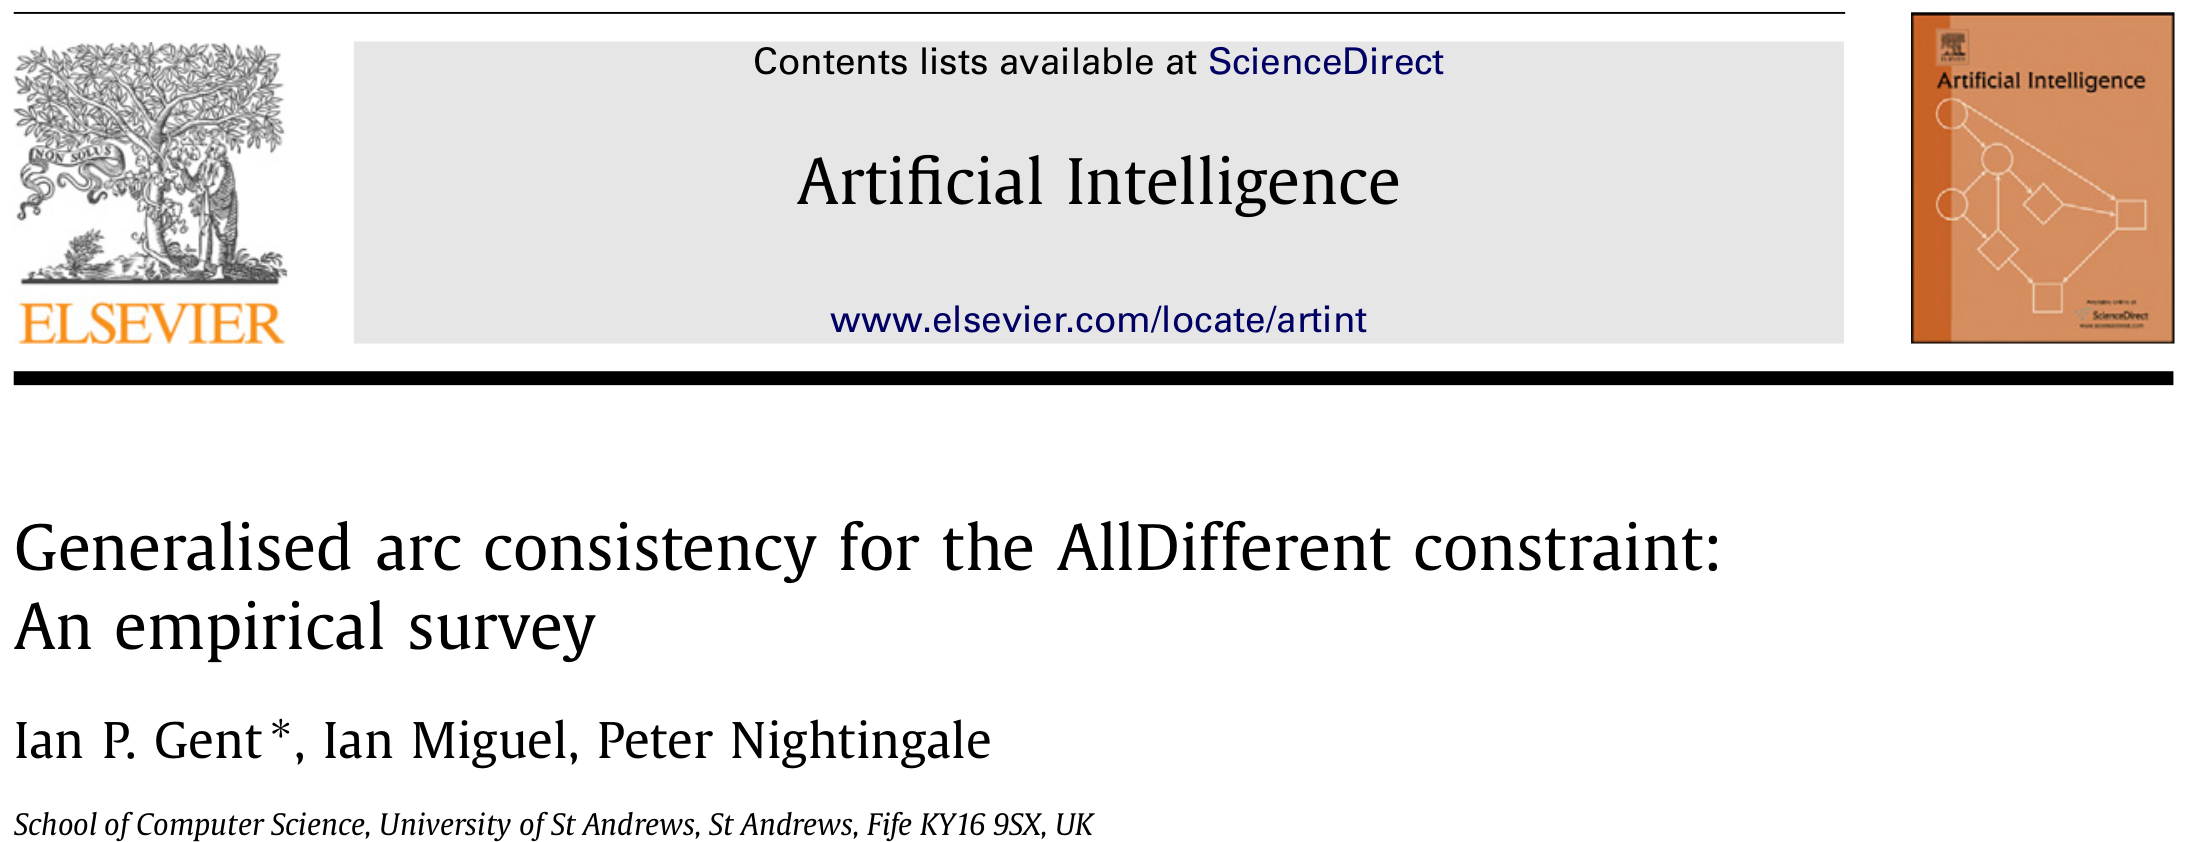
\includegraphics[scale=0.12]{alldifftitle.png}}%
    \only<2>{\centering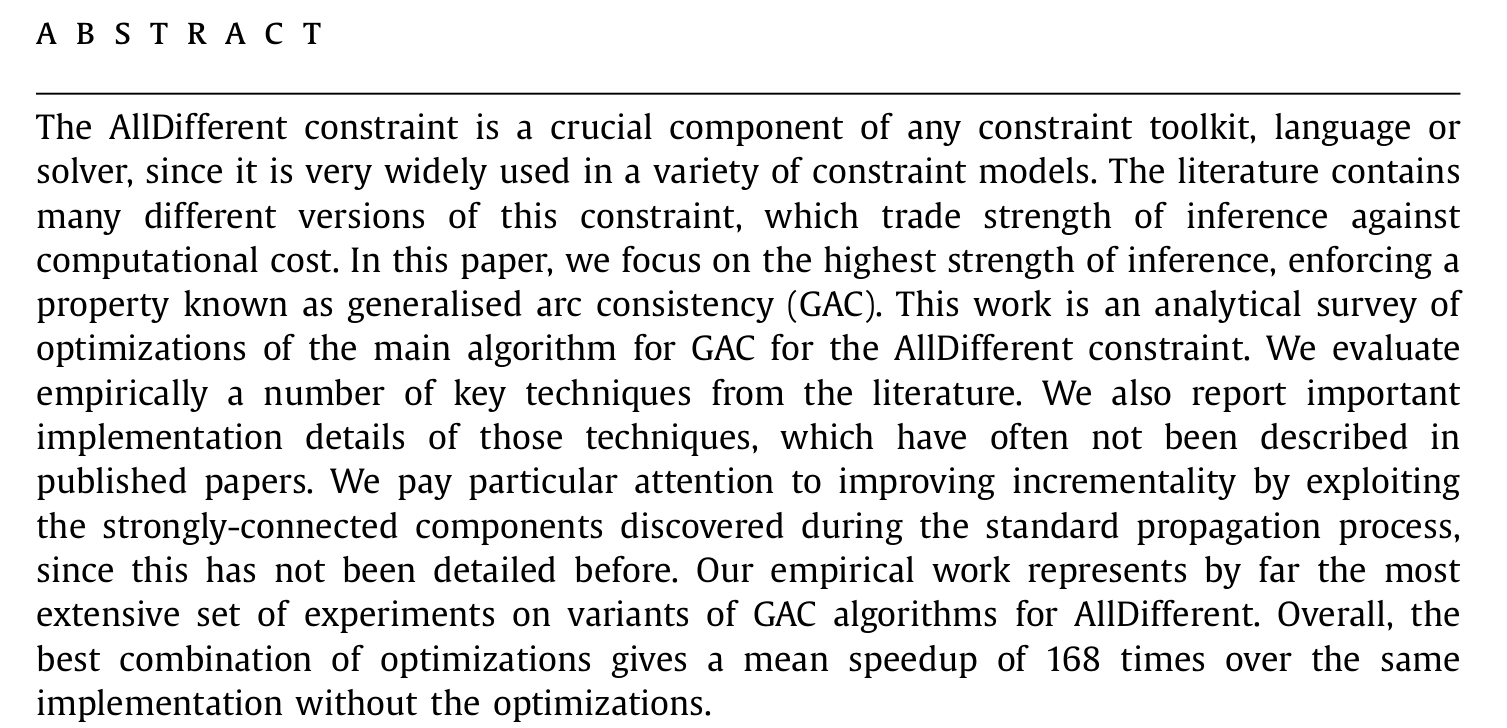
\includegraphics[scale=0.15]{alldiffabstract.png}}%
\end{frame}

\begin{frame}[fragile]{A Sudoku Solver in Choco}
    \only<1>{\lstinputlisting[basicstyle=\scriptsize\ttfamily]{code/herald20061222E.txt}}
    \only<2>{\lstinputlisting[language=Java, basicstyle=\scriptsize\ttfamily, keywordstyle=\color{uofgcobalt}]{code/Sudoku-1-snippet.java}
        }
    \only<3>{\lstinputlisting[language=Java, basicstyle=\scriptsize\ttfamily, keywordstyle=\color{uofgcobalt}]{code/Sudoku-2-snippet.java}
        }
    \only<4-5>{\lstinputlisting[language=Java, basicstyle=\scriptsize\ttfamily, keywordstyle=\color{uofgcobalt}]{code/Sudoku-3-snippet.java}
        \begin{tikzpicture}[remember picture, overlay]
            \node [anchor=north east, xshift=-0.5cm, yshift=-1cm] at (current page.north east) {
                \only<5>{
\includegraphics[keepaspectratio=true,scale=0.45]{eww.jpg}}
            };
        \end{tikzpicture}
        }
    \only<6>{\lstinputlisting[language=Java, basicstyle=\scriptsize\ttfamily, keywordstyle=\color{uofgcobalt}]{code/Sudoku-4-snippet.java}}
    \only<7>{\lstinputlisting[language=Java, basicstyle=\scriptsize\ttfamily,
    keywordstyle=\color{uofgcobalt}]{code/Sudoku-5-snippet.java}}
\end{frame}

\begin{frame}[t]{Some Experiments}
    \only<1> {
        \lstinputlisting[basicstyle=\scriptsize\ttfamily]{code/herald20061222E.txt}
    }
    \only<2-4> {
        \begin{columns}
            \begin{column}{0.45\textwidth}
                Using not-equals:
                \lstinputlisting[basicstyle=\scriptsize\ttfamily]{code/herald20061222E-neq.txt}
            \end{column}
            \begin{column}{0.45\textwidth}
                \only<3->{
                    Using all-different:
                    \lstinputlisting[basicstyle=\scriptsize\ttfamily]{code/herald20061222E-alldiff.txt}
                }
            \end{column}
        \end{columns}
        \only<4->{
            Both solved without guessing (Nodes: 1). Using not equals is 1ms faster to set up and
            1ms faster to solve. We could run it lots of times to test for statistical significance,
            but do we care?
        }
    }

    \only<5> {
        \lstinputlisting[basicstyle=\scriptsize\ttfamily]{code/herald20061222H.txt}
    }
    \only<6-8> {
        \begin{columns}
            \begin{column}{0.45\textwidth}
                Using not-equals:
                \lstinputlisting[basicstyle=\scriptsize\ttfamily]{code/herald20061222H-neq.txt}
            \end{column}
            \begin{column}{0.45\textwidth}
                \only<7->{
                    Using all-different:
                    \lstinputlisting[basicstyle=\scriptsize\ttfamily]{code/herald20061222H-alldiff.txt}
                }
            \end{column}
        \end{columns}
        \only <8->{
            All-different can solve without guessing (Nodes: 1 vs 20) but is 2ms slower to run and
            8ms slower to set up.
        }
    }

    \only<9> {
        \lstinputlisting[basicstyle=\scriptsize\ttfamily]{code/times20070107.txt}
    }
    \only<10-12> {
        \begin{columns}
            \begin{column}{0.45\textwidth}
                \lstinputlisting[basicstyle=\scriptsize\ttfamily]{code/times20070107-neq.txt}
            \end{column}
            \begin{column}{0.45\textwidth}
                \only<11->{
                    \lstinputlisting[basicstyle=\scriptsize\ttfamily]{code/times20070107-alldiff.txt}
                }
            \end{column}
        \end{columns}
        \only <12>{
            Less guessing from all-different again, and it's slightly faster.
        }
    }

    \only<13> {
        \lstinputlisting[basicstyle=\scriptsize\ttfamily]{code/times20071015.txt}
    }
    \only<14-16> {
        \begin{columns}
            \begin{column}{0.45\textwidth}
                Using not-equals:
                \lstinputlisting[basicstyle=\scriptsize\ttfamily]{code/times20071015-neq.txt}
            \end{column}
            \begin{column}{0.45\textwidth}
                \only<15->{
                    Using all-different:
                    \lstinputlisting[basicstyle=\scriptsize\ttfamily]{code/times20071015-alldiff.txt}
                }
            \end{column}
        \end{columns}
        \only <16>{
            Things aren't looking good for all-different\ldots
        }
    }

    \only<17> {
        \centering\vspace*{-1.5em}
        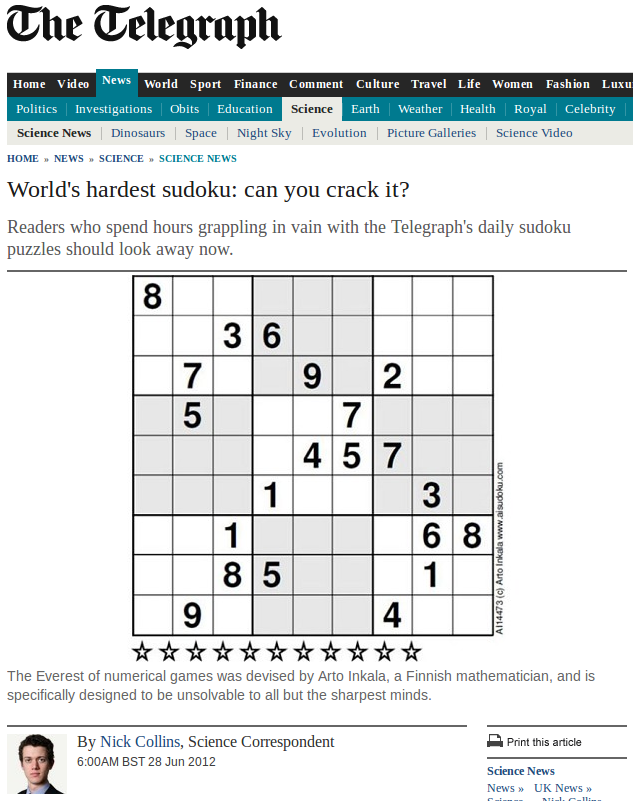
\includegraphics[keepaspectratio=true,scale=0.24]{hardest.png}
    }
    \only<18-20> {
        \begin{columns}
            \begin{column}{0.45\textwidth}
                Using not-equals:
                \lstinputlisting[basicstyle=\scriptsize\ttfamily]{code/hardest-neq.txt}
            \end{column}
            \begin{column}{0.45\textwidth}
                \only<19->{
                    Using all-different:
                    \lstinputlisting[basicstyle=\scriptsize\ttfamily]{code/hardest-alldiff.txt}
                }
            \end{column}
        \end{columns}
        \only <20>{
            Finally, an epic and extremely convincing victory for all-different, we saved an entire
            47ms overall.
        }
    }

    \only<21> {
        \scalebox{0.7}{
            \begin{minipage}{2\paperwidth}
                \lstinputlisting[basicstyle=\fontsize{5pt}{6pt}\ttfamily]{code/huge.txt}
        \end{minipage}}
    }

    \only<22-24> {
        \begin{columns}[t]
            \begin{column}{0.45\textwidth}
                Using not-equals:
                \lstinputlisting[basicstyle=\scriptsize\ttfamily]{code/huge-neq.txt}
            \end{column}
            \begin{column}{0.45\textwidth}
                \only<23-> {
                    Using all-different:
                    \lstinputlisting[basicstyle=\scriptsize\ttfamily]{code/huge-alldiff.txt}
                }
            \end{column}
        \end{columns}
        \only<24>{
            Given Nodes: 1, nothing clever is needed to solve this, so a really bored human
            could probably do this faster than the not-equals version.}
    }
\end{frame}

\begin{frame}{Do Global Constraints Always Help?}
    \begin{itemize}
        \item Sometimes globals make a spectacular difference.

        \item Sometimes global constraints end up not giving any more deletions than their
            decompositions, and can take longer to propagate. Sometimes extra deletions don't help
            anyway.

        \item Some global constraints only have weaker propagators: GAC can be too hard to be
            practical, or \NP-complete on its own.

        \item It is impossible to get GAC for all-different from a polynomial-sized SAT encoding.

        \item Using globals isn't a \emph{guaranteed} benefit, but they make the model easier to
            read, and it's easier to translate from globals to decompositions and encodings than the
            other way around.
    \end{itemize}
\end{frame}

\begin{frame}{Consistency, Again}
    \begin{itemize}
        \item Consistency depends upon how exactly your constraints are specified.
        \item GAC is the strongest possible consistency level, if all we can do is consider one
            constraint at once and delete values from domains.
    \end{itemize}
\end{frame}

\begin{frame}{Are You Smarter than a Constraint Solver?}
    \only<1> {
        \begin{center}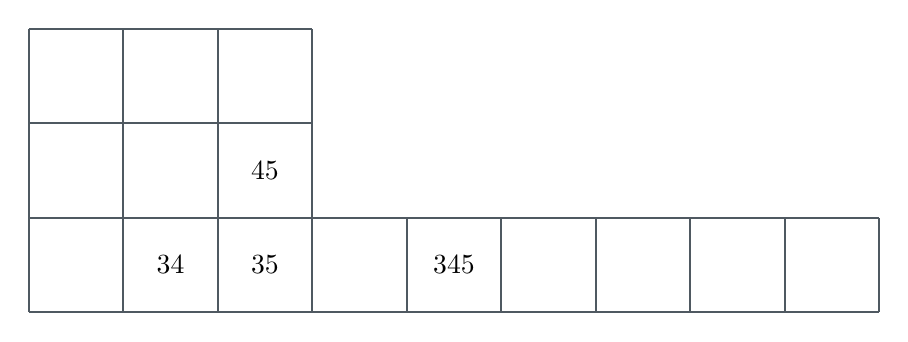
\begin{tikzpicture}[scale=0.4]
            \draw[thick, scale=3, color=uofgslate] (0, 0) grid (3, 3);
            \draw[thick, scale=3, color=uofgslate] (3, 0) grid (9, 1);

            \node[anchor=center] at (4.5, 1.5) { 34 };
            \node[anchor=center] at (7.5, 1.5) { 35 };
            \node[anchor=center] at (7.5, 4.5) { 45 };
            \node[anchor=center] at (13.5, 1.5) { 345 };

        \end{tikzpicture}\end{center}
    }

    \only<2> {
        \begin{itemize}
            \item Remember: propagation only considers \emph{one constraint at a time}, and the only
                communication between constraints is by deleting values.

            \item Automatically combining certain constraints is an active research topic.
                \begin{itemize}
                    \item But getting ``the best possible'' filtering from two ``all different''
                        constraints simultaneously is \NP-hard\ldots
                \end{itemize}
        \end{itemize}
    }
\end{frame}

\begin{frame}{Not the Exam Question Because There is No Exam}

    What is a \emph{Hall set}, and why is it useful for propagation? Use the following model to
    illustrate your answer:
    \begin{align*}
        & x_1 \in \{ 4, 5 \}   && x_2 \in \{ 1, 2, 3, 4 \}  && x_3 \in \{ 3, 4, 5 \} \\
        & x_4 \in \{ 5, 6 \}   && x_5 \in \{ 3, 5 \} \\
        & \mathrlap{\textit{alldifferent}( x_1, x_2, x_3, x_4, x_5 )}
    \end{align*}

    Suppose our solver did not have an ``all different'' constraint. Show how to rewrite this model
    using only binary constraints.  What effect would this have on propagation? \\[0.2cm]

    Aside from propagation, describe another benefit of global constraints.

\end{frame}

\section{Linear Constraints}

\begin{frame}{Linear (or Scalar) Products}
    \begin{itemize}
        \item Let $c$ be an array of constants and $v$ an array of variables. The \emph{scalar
            product} of $c$ and $v$ is \begin{align*}
        c \cdot v = \sum_{i \in A}{c[i] \times v[i]}\end{align*}
        \item We constrain this with an operator to another variable (or constant). The operator can
            be an equation ($=$), or an inequality ($\le$ or $\ge$).
        \item In MiniZinc, the compiler automatically detects constraints like $3 * x + 2 * y <= 10$
            and $sum(i \operatorname{in} s)(a[i] * b[i]) = 12$.
        \item These are known as \emph{linear} equalities and inequalities, because
            geometrically they define a straight line.
    \end{itemize}
\end{frame}

\begin{frame}{What Can We Do?}
    \vspace*{-1em}
    \begin{align*}
        & x_1 \in \{ 0, 2 \} \\
        & x_2 \in \{ 0, 1 \} \\
        & x_3 \in \{ 0, 2 \} \\
        & 5x_1 + 2x_2 + x_3 \ge 8
    \end{align*}

    \begin{itemize}
        \item <2-> $x_1$ must be at least $1$, because we can get at most $(2 *
            1) + (1 * 2) = 4$ from the other two variables.
        \item <3-> $x_2$ and $x_3$ don't change, because $x_1 = 2$ can satisfy the inequality on its own.
        \item <4-> What if $x_1 \in \{ 0, 1 \}$?
            \begin{itemize}
            \item <5-> $x_2$ can't be $0$, because we can only get $(5 * 1) + (1 * 2) = 7$ from the other two
                without its help.
            \item <6-> $x_3$ can't be $0$, because we can only get $(5 * 1) + (2 * 1) = 7$ from the other two
                variables without its help.
            \end{itemize}
    \end{itemize}
\end{frame}

\begin{frame}{The Slack Algorithm for $\ge$ Inequalities}
    \begin{itemize}
        \item Feasibility: if every variable contributes as much as possible,
            do we have enough?
        \item Filtering: for each variable in turn, what's the most the
            remaining variables can contribute, and how much do I have to
            contribute if this happens?
            \begin{itemize}
                \item Assuming only positive numbers, this might increase lower bounds.
            \end{itemize}
        \item Actual algorithm removed for mental health reasons\ldots
    \end{itemize}
\end{frame}

\begin{frame}{When Do Linear Inequalities Propagate?}
    \begin{itemize}
        \item For positive coefficients and $\ge$: only when an upper bound changes.
        \item Can be even more specific sometimes\ldots
            \begin{itemize}
                \item For example, if one variable gets a very large value, maybe
                    the constraint will always be satisfied.
            \end{itemize}
    \end{itemize}
\end{frame}

\begin{frame}[fragile]{In Choco}
    \only<1> {
        \lstinputlisting[language=Java, basicstyle=\scriptsize\ttfamily, keywordstyle=\color{uofgcobalt}]{code/Scalar-snippet.java}
    }
    \only<2> {
        \begin{minipage}{0.47\paperwidth}\lstinputlisting[basicstyle=\scriptsize\ttfamily]{code/Scalar-output.txt}
        \end{minipage}\begin{minipage}{0.44\paperwidth}\lstinputlisting[basicstyle=\scriptsize\ttfamily]{code/Scalar-output2.txt}
        \end{minipage}
    }
\end{frame}

\begin{frame}{Remember Generalised Arc Consistency?}
    \begin{minipage}{0.6\paperwidth}
    \begin{itemize}
        \item A \emph{binary} constraint is arc consistent if we can pick any value from either of its
            two variables, and find a supporting value in the other variable.
        \item A global constraint is generalised arc consistent (GAC) if each value
            is present in at least one solution to the constraint.
        \item Enforcing GAC will only touch upper and lower bounds for
            linear inequalities.
            \begin{itemize}
                \item We could also define \emph{bounds} consistency.
            \end{itemize}
    \end{itemize}
    \end{minipage}\begin{minipage}{0.4\paperwidth}
        \hspace*{-1cm}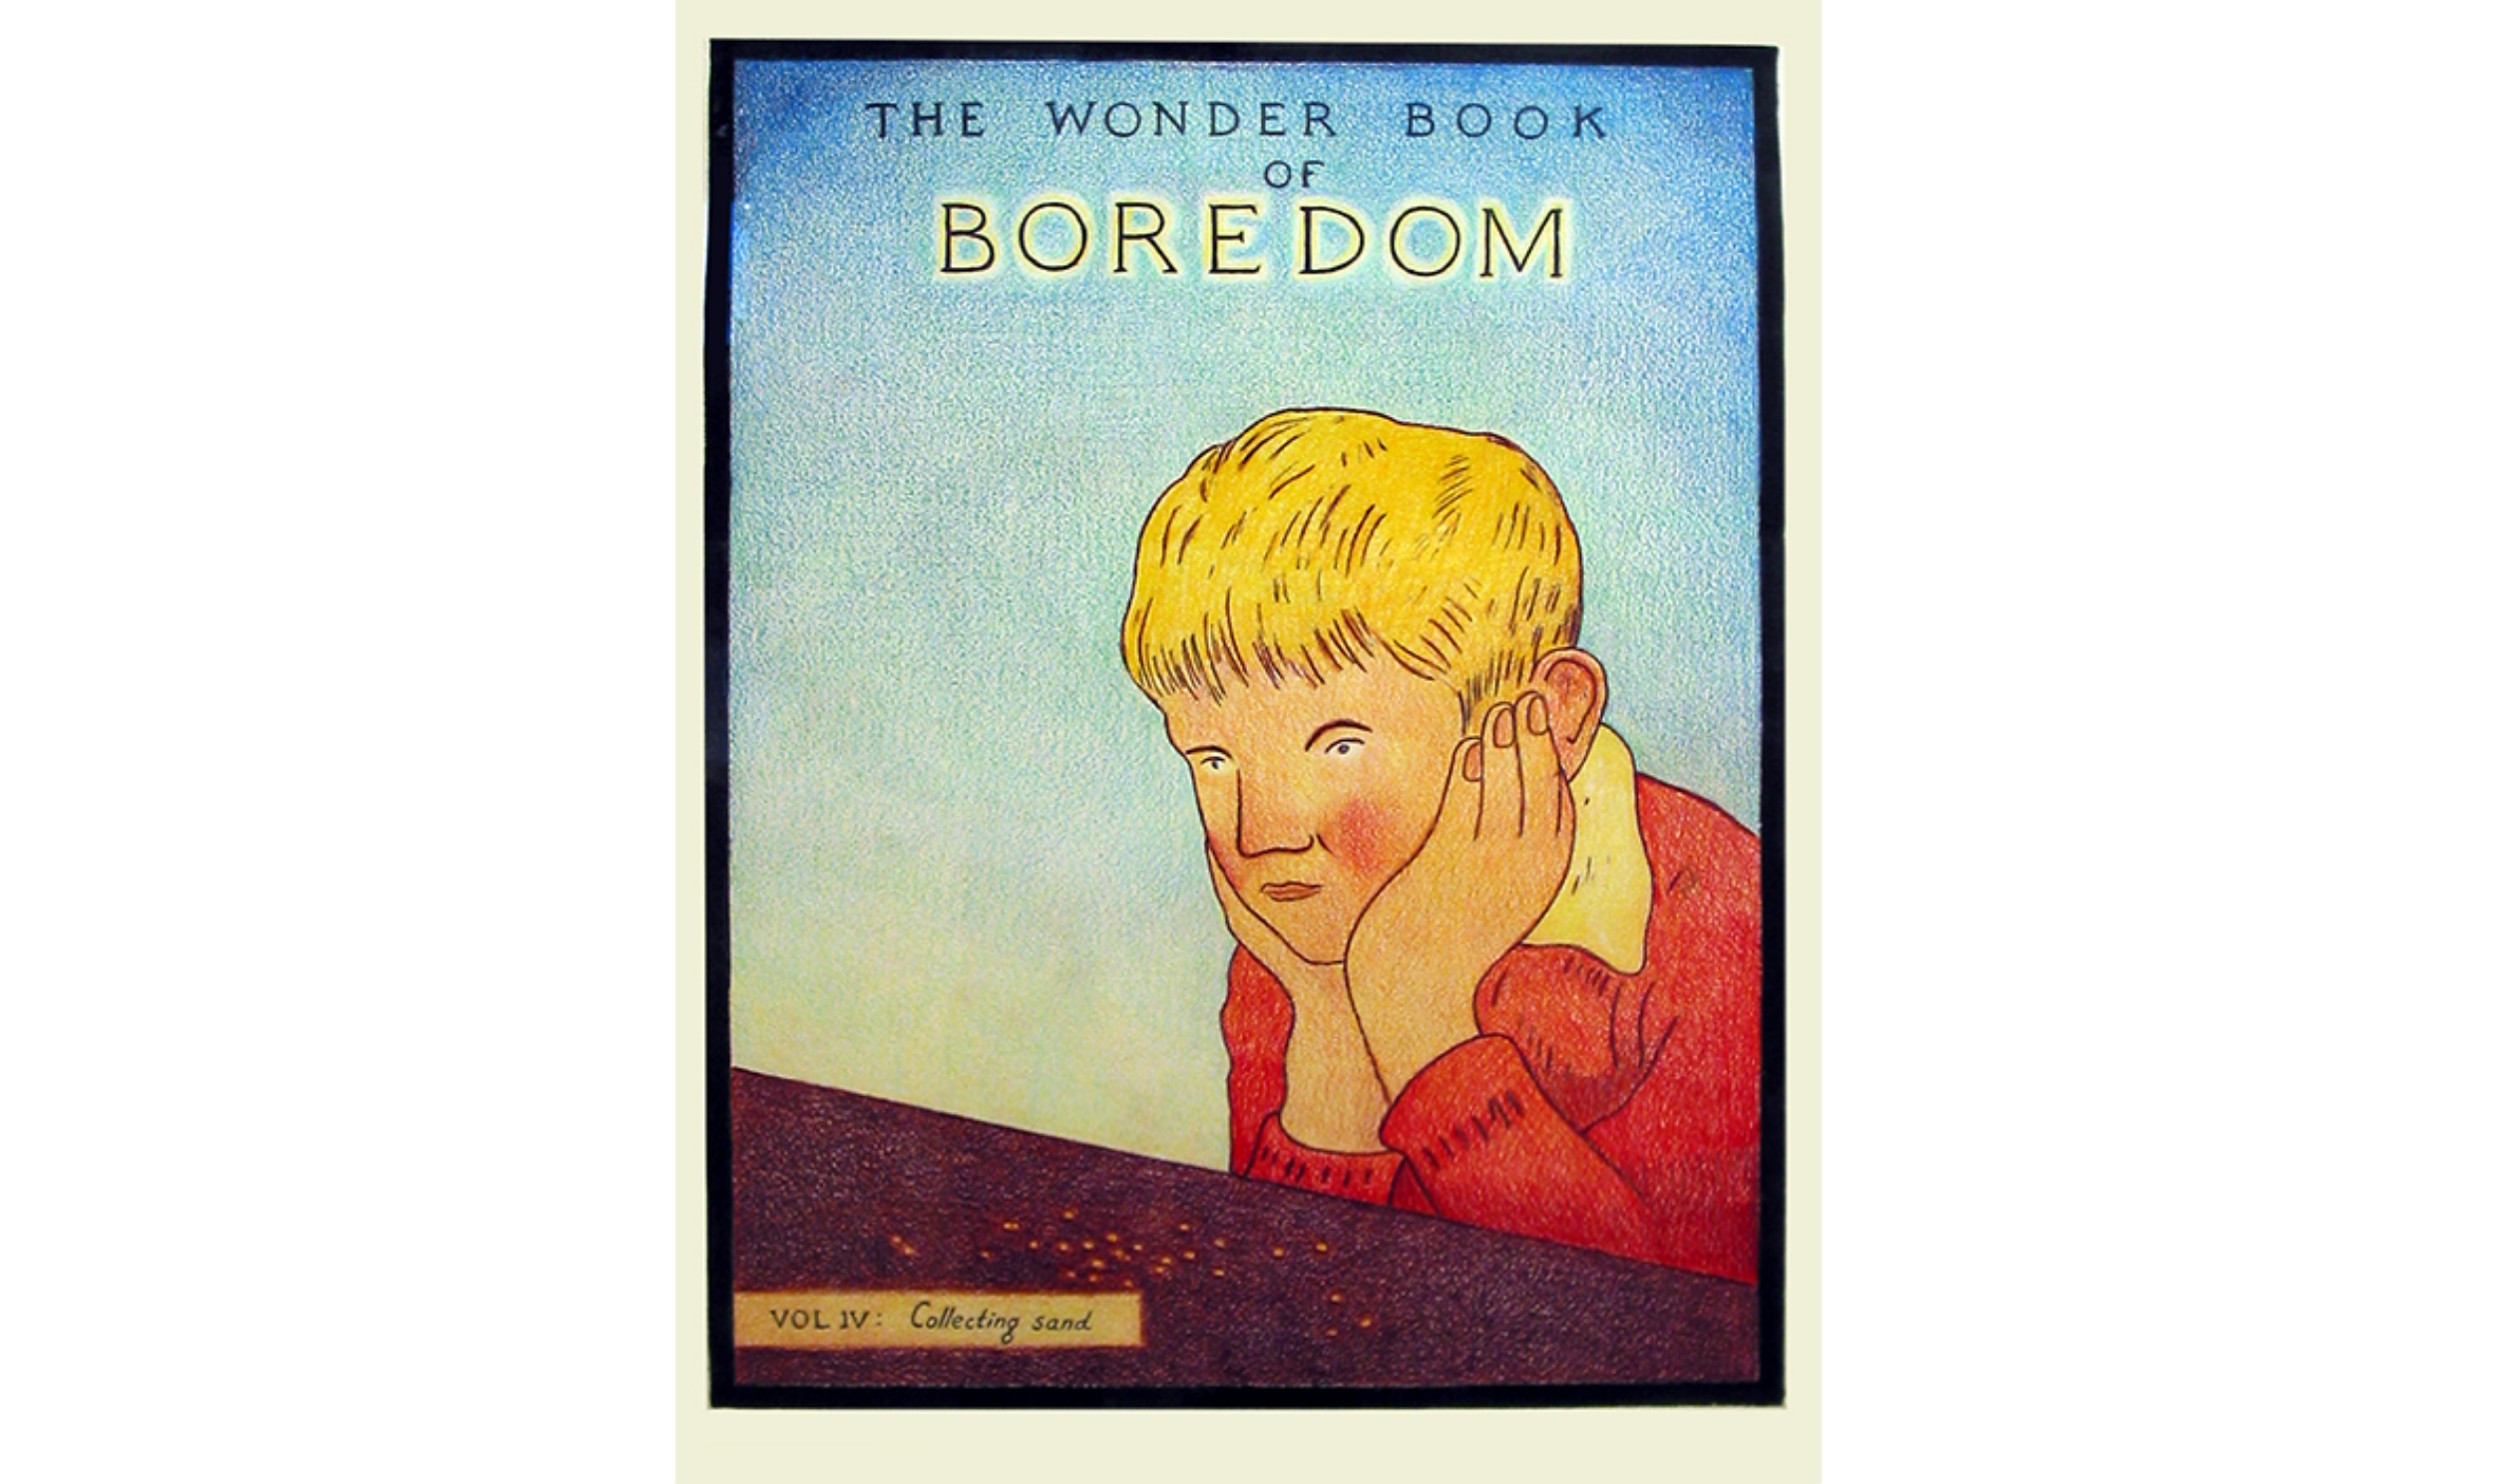
\includegraphics[keepaspectratio=true,scale=0.07]{bored.png}
    \end{minipage}
\end{frame}

\begin{frame}{Linear Equalities}
    \begin{itemize}
        \item What if we have an equation, rather than an inequality?
            \begin{align*}x = \sum_{i \in A}{c[i] \times v[i]}\end{align*}
        \item <2-> The subset sum problem is \NP-complete\ldots
        \item <3-> We can enforce GAC on a $\le$ constraint and a $\ge$
            constraint simultaneously. This is \textbf{not} the same as enforcing GAC
            on the equality.
    \end{itemize}
\end{frame}

\begin{frame}[t,fragile]{In Choco}
    \only<1> {
        \lstinputlisting[language=Java, basicstyle=\scriptsize\ttfamily, keywordstyle=\color{uofgcobalt}]{code/SmallScalarEquality-snippet.java}
    }
    \only<2-3> {
        \lstinputlisting[basicstyle=\scriptsize\ttfamily]{code/SmallScalarEquality-output.txt}
        \only<3->{Somehow it's figured out the constraint is infeasible, and it says our constraint
        is a Table, not a Sum.}
    }
\end{frame}

\begin{frame}{In Choco (Attempt Two)}
    \only<1> {
        Let's try some bigger numbers and see what happens.
        \lstinputlisting[language=Java, basicstyle=\scriptsize\ttfamily, keywordstyle=\color{uofgcobalt}]{code/BigScalarEquality-snippet.java}
    }
    \only<2> {
        \begin{minipage}{0.47\paperwidth}\lstinputlisting[basicstyle=\scriptsize\ttfamily]{code/BigScalarEquality-output.txt}
        \end{minipage}\begin{minipage}{0.44\paperwidth}\lstinputlisting[basicstyle=\scriptsize\ttfamily]{code/BigScalarEquality-output2.txt}
        \end{minipage}
    }
\end{frame}

\begin{frame}{When Do Linear Equalities Propagate?}
    \begin{itemize}
        \item As a pair of inequalities, when bounds change.
        \item For GAC, it's complicated\ldots
    \end{itemize}
\end{frame}

\begin{frame}{I'm Telling You This Twice Because It's Important}
    \begin{itemize}
        \item Propagation and consistency both depend upon how exactly you represent constraints.
        \item Modelling languages and solvers will \emph{sometimes} help you out.
    \end{itemize}
\end{frame}

\begin{frame}{Jess Probably Isn't Mean Enough To Ask This On A Test}

    Consider the following constraint:
    \begin{align*}
        2x_1 - 2x_2 + 4x_3 \ge 11
    \end{align*}
    Given $x_1 \in \{ 2, 3, 4, 5 \}$, $x_2 \in \{ 1, 2, 3, 50 \}$ and $x_4 \in \{ 0, 1, 2
    \}$, prove $x_2 \ne 50$. What else can we infer?

    Now suppose we add a second constraint,
    \begin{align*}
        2x_1 - 2x_2 + 4x_3 \le 11
    \end{align*}
    Why is enforcing consistency on these two constraints \emph{not} the same as enforcing
    consistency on this single equality constraint?
    \begin{align*}
        2x_1 - 2x_2 + 4x_3 = 11
    \end{align*}

\end{frame}

\section{Extensional (Table) Constraints}

\begin{frame}{Table Constraints}
    \begin{itemize}
        \item We can represent a constraint as a list of permitted
            tuples: \[ [A, B, C] \in \{ [1, 2, 3], [1, 3, 2], [2, 1, 3], [2, 3,
            1], [3, 1, 2], [3, 2, 1] \} \]
        \item This is the preferred definition for theoretical computer
            science, but not commonly used in practice.
        \item Sometimes table constraints \emph{are} the best option, though.
    \end{itemize}
\end{frame}

\begin{frame}{Consistency, Round Three}
    \begin{itemize}
        \item Back to generalised arc consistency!
        \item Call a tuple \emph{feasible} if each of its values remains in the
            domain of its respective variable.
        \item If each value in each variable is present in at least one
            feasible tuple, we have GAC.
    \end{itemize}
\end{frame}

\begin{frame}{Propagating Table Constraints}
    \begin{itemize}
        \item Keep track of remaining feasible tuples.
        \item For example, by using an additional ``variable'', \begin{align*}
                T = 1 \rightarrow{} &(A = 1 \land B = 2 \land C = 3) \\
                T = 2 \rightarrow{} &(A = 1 \land B = 1 \land C = 2) \\
                T = 3 \rightarrow{} &(A = 2 \land B = 1 \land C = 3) \\
                T = 4 \rightarrow{} &(A = 2 \land B = 3 \land C = 1) \\
                T = 5 \rightarrow{} &(A = 3 \land B = 1 \land C = 2) \\
                T = 6 \rightarrow{} &(A = 3 \land B = 2 \land C = 1)
        \end{align*}
        \item Remove any value that is not supported in a feasible tuple.
    \end{itemize}
\end{frame}

\begin{frame}{Why Not Just Use Table Constraints?}
    \begin{itemize}
        \item We can propagate table constraints in (low) polynomial time, and get GAC.
            \begin{itemize}
                \item There are much faster algorithms than the one on the
                    previous slide.
                \item See: one of the suggested poster papers.
            \end{itemize}
        \item Why not use table constraints for everything?
        \item <2-> Tables can be exponentially long, e.g. for all-different.
            \begin{itemize}
                \item <2-> Would it be possible to redo the Sudoku experiments
                    using table constraints?
            \end{itemize}
    \end{itemize}
\end{frame}

\begin{frame}{Autotabulation}
    \begin{itemize}
        \item Remember Choco being clever with linear equalities?
        \item A solver can turn one or more constraints into a table constraint
            to get more powerful propagation.
        \item If you know when to do this, it can be really powerful.
        \item See: one of the suggested poster papers.
    \end{itemize}
\end{frame}

\begin{frame}{Beyond Table Constraints}
    \begin{itemize}
        \item Smart tables: wildcards, negations, and ranges.
            \begin{itemize}
                \item Can make tables much smaller for some problems.
            \end{itemize}
        \item Decision diagrams.
            \begin{itemize}
                \item Even more compact representations.
            \end{itemize}
        \item Regular expressions.
            \begin{itemize}
                \item See: one of the suggested poster papers.
            \end{itemize}
    \end{itemize}
\end{frame}

\begin{frame}[fragile]{Shift Pattern Scheduling}
    \vspace*{-0.5em}%
    \only<1>{
        \begin{itemize}
            \item Produce a schedule for eleven employees for two weeks.
            \item Each employee can be on day shift, night shift, or off.
            \item Four employees present on each day shift.
            \item Two employees present on each night shift.
            \item Can't work more than five day shifts in a row.
            \item Can't work more than two night shifts in a row.
            \item Day shift can only be followed by a day shift or a day off.
            \item Night shift can only be followed by a night shift or a day off.
        \end{itemize}
    }%
    \only<2>{\lstinputlisting[basicstyle=\tiny\ttfamily]{code/yaycapitalism1.mzn}}%
    \only<3-4>{\lstinputlisting[basicstyle=\tiny\ttfamily]{code/yaycapitalism1-out.txt}
    \uncover<4>{Those last two employees might not be very happy\ldots}}%
    \only<5>{\lstinputlisting[basicstyle=\tiny\ttfamily]{code/yaycapitalism2.mzn}}%
    \only<6>{\lstinputlisting[basicstyle=\tiny\ttfamily]{code/yaycapitalism2-out.txt}}%
\end{frame}

\begin{frame}{Ethical Considerations}
    \begin{itemize}
        \item Easy to write a model that produces a valid schedule.
        \item Hard to write a \emph{good} model that doesn't ruin people's lives.
            \begin{itemize}
                \item \emph{Balance} constraints for minimum and maximum hours.
                \item Optimise to respect employee preferences.
            \end{itemize}
        \item <2-> Ethical obligation to support our democratically elected
            capitalist government by maximising shareholder value:
            \begin{itemize}
                \item <2-> Give fewest hours to most expensive (or least productive) employees?
                \item <2-> No need to lay anyone off, just use zero hour contracts.
                \item <2-> Get rid of poorly performing employees by giving them
                    bad shift patterns.
            \end{itemize}
    \end{itemize}
\end{frame}

\begin{frame}[plain,noframenumbering]
    \begin{tikzpicture}[remember picture, overlay]
        \node at (current page.north west) {
            \begin{tikzpicture}[remember picture, overlay]
                \fill [fill=uofguniversityblue, anchor=north west] (0, 0) rectangle (\paperwidth, -1.7cm);
            \end{tikzpicture}
        };

        \node (logo) [anchor=north east, shift={(-0.3cm,-0.2cm)}] at (current page.north east) {
            
\includegraphics[keepaspectratio=true,scale=0.55]{UoG_keyline.pdf}
        };
    \end{tikzpicture}
\end{frame}

\end{document}

